\subsection{Radiation Monitoring System Design}
\label{sec:Radiation Design}
The Raspberry Pi has proven to operate at float altitudes both from the previous SORA flight and other HASP payloads from previous years and as such was chosen again to host the control and analysis software. Similarly to the SORA 1.0 flight, both TimePIX devices were interfaced with the RPI via USB and controlled via the pypixet library developed at CERN by (Daniel Turcek?). The major difference for the 2018 SORA flight is that the software was redesigned to support an arbitrary number of TimePIX devices to record data at the same time. This means that multiple TimePIX detector experiments could be run concurrently without adding another control system. Another major difference is that the detectors could be configured directly from the serial uplink and collected data could be downlinked in real time. This allowed data from the detector to be analyzed and plotted in real time by the members of our team.

The control and analysis software was written entirely in Python and operated directly on top of the default Raspbian image. Because the pypixet software blocks when exposing the detector for collection, both detectors had to collect data in their own threads to allow the main thread to process uplink commands and control other systems. Data from each of these threads was then placed onto a queue where the main thread could periodically check if there was data ready to be processed. When a frame from one of the detectors was ready to be processed the main thread performed the analysis and then downlinked the results. Consequently, downlink speed was directly tied to shutter speed. An overview of the software design is shown in Figure (INSERT REFERENCE HERE)
%\ref{softwaredesign}.THIS WAS MOVED HERE SINCE IT WAS AFFECTING THE COMPILER - NEEDS TO BE PROPERLY DEFINED

\begin{figure}[h!]
	\begin{center}
	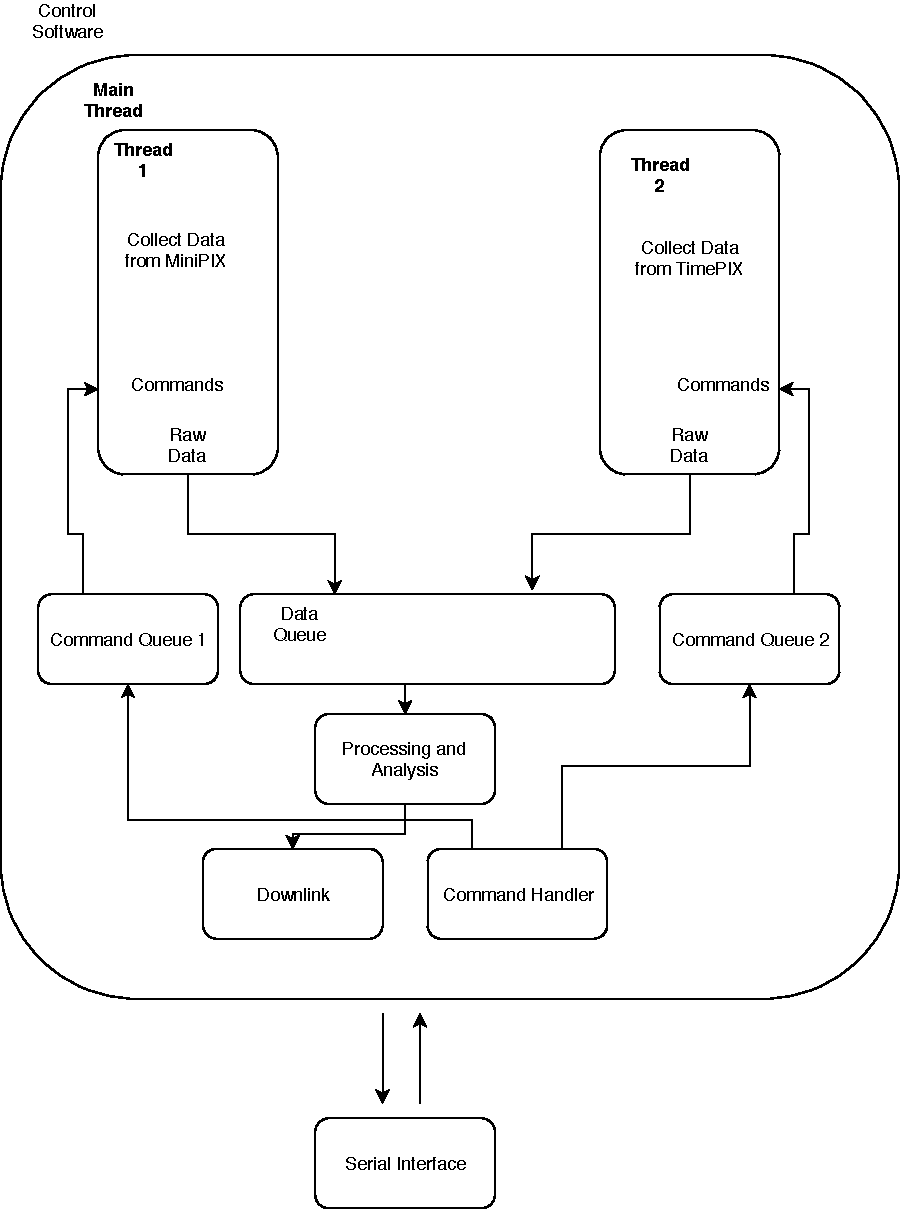
\includegraphics[width=0.5\textwidth]{figures/SoftwareDesign.pdf}
	\caption{Software design for the radiation control systems.}
	\label{softwaredesign}
	\end{center}
\end{figure}
\clearpage
 
By and large the MiniPIX, and TimePIX detectors have proven to be robust and resilient towards large thermal fluctuations. However, during the course of integration testing in Palestine a failure was observed. During the cold cycle of the test a slow but steadily increasing number of counts was observed that is anomalous to what one would expect near the earths surface. The expected number of counts per second should've been close to 3 but the downlinked data was reporting values of over 300 as shown in Figure (INSERT FIGURE REFERENCE HERE)
%\ref{integrationtemps}.  THIS WAS MOVED HERE SINCE IT WAS AFFECTING THE COMPILER - NEEDS TO BE PROPERLY DEFINED
A correlation analysis was performed and showed that there was no direct correlation between device counts and temperature. Additionally, this behavior was not observed on an identical detector used during the 2017 SORA flight. 

After consulting with some of the members of the TimePIX collaboration at the University of Houston and NASA we were informed that they were unable to determine a concrete reason for the failure but did provide a couple of possible explanations. The first, but most unlikely cause is that of a single event upset in the device causing the detector threshold to be lowered. TimePIX devices deployed on the International Space Station often experience this kind of behavior and consequently reload their configurations every few frames to prevent it. This is an exceedingly unlikely possibility in our case however, given the low levels of high energy particles near the earths surface. Another possibility is that the cold caused a partial failure in the power supply and the RPI was unable to provide enough power to the detector. This explanation is somewhat more likely, but because this kind of failure was never observed again it is difficult to say definitively what the cause was.

\begin{figure}[h!]
	\begin{center}
	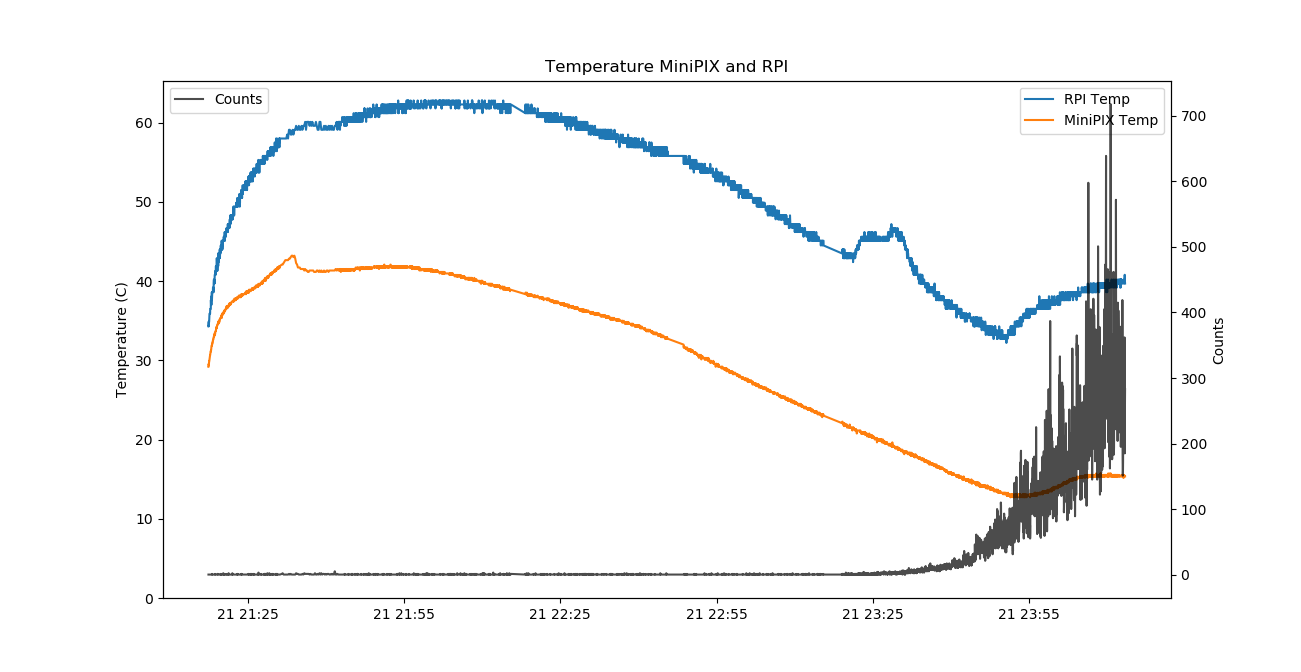
\includegraphics[width=\textwidth]{figures/tempsandcountsvtime.png}
	\caption{Temperature of flight computer and detector and counts.}
	\label{integrationtemps}
	\end{center}
\end{figure}

\subsection{Telemetry}
\label{sec:Telemetry}

All telemetry was handled via the RPi. The DB9 interface from the HASP Large Payload plate was converted to a 
RS-232 female plug. A Male RS 232 to Male USB \ref{fig:rs232-usb} was used to connect it to a USB port of the RPi. 
The downlink data packets were written to describe the radiation data. 
The uplink commands were sent to the RPi which delegated the work either to itself or the Arduino which 
was connected to the RPi via USB as shown in figure \ref{fig:telem-diagram}.

\begin{figure}[h!]
\centering
\begin{minipage}{.5\textwidth}
  \centering
  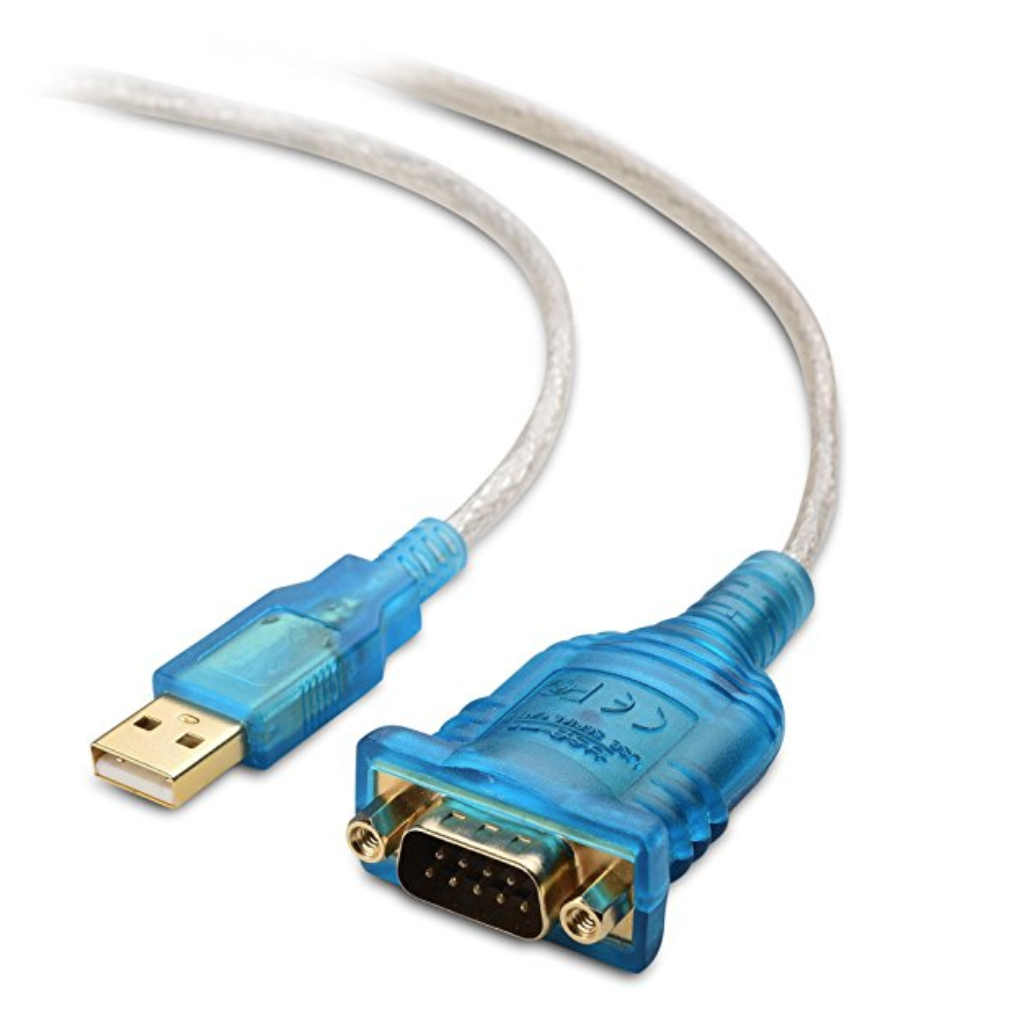
\includegraphics[width=.4\linewidth]{figures/rs232tousb.png}
  \caption{RS 232 to Male USB}{Cable used to connect the DB9 interface to the RPi}
  \label{fig:rs232tousb}
\end{minipage}
\begin{minipage}{.5\textwidth}
  \centering
  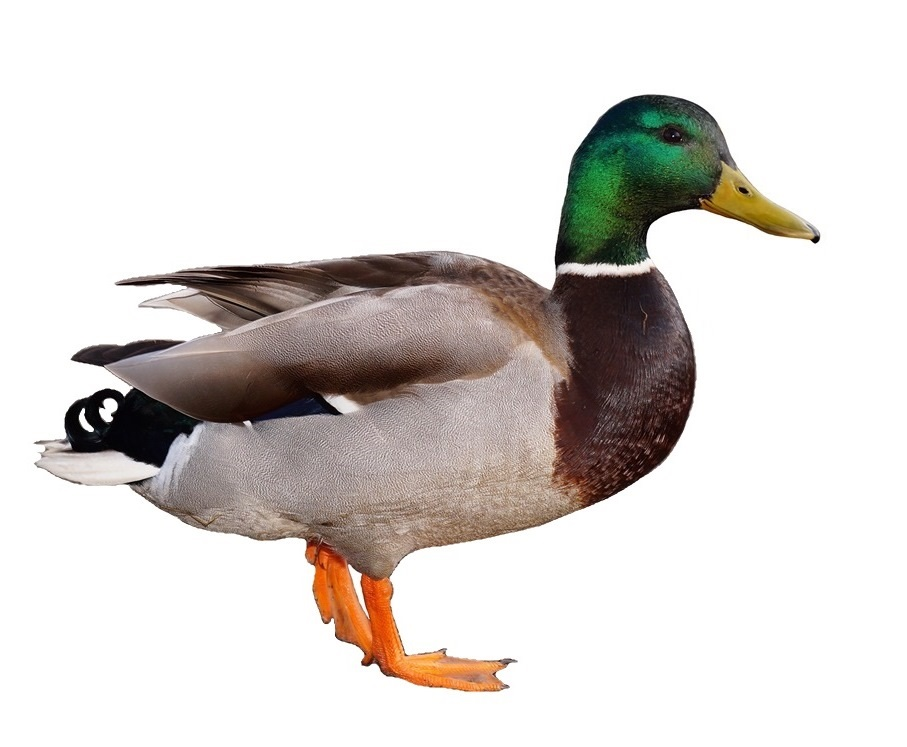
\includegraphics[width=.4\linewidth]{figures/duck.jpg}
  \caption{Telemetry}{Diagram depicting how telemetry was processed}
  \label{fig:telem-diagram}
\end{minipage}
\end{figure}

\subsubsection{Uplink}
\label{sec:Uplink} 
Uplink commands were used to start, end, and change parameters within our payload over the course of flight. 
Table \ref{All-Commands} list the uplink commands, thier functions and a brief description of what they did. 

\subsubsection{Downlink}
\label{sec:Downlink}
Downlink data was written to describe the data being read from the MiniPix detector. 

\begin{table}[h!]
\centering
\caption{Table of All Uplink Commands Used During Flight}
\label{tab:All-Commands}
\bigskip
\begin{tabular}{c|c|c|c}
\hline
\hline
\multicolumn{1}{c|}{\bfseries Command} & \multicolumn{1}{c|}{\bfseries Byte 1} &  \multicolumn{1}{c|}{\bfseries Byte 2} & \multicolumn{1}{c}{\bfseries Expected Current Consumption} \\
\hline
    	Start Acquisition  	& 0x01	& -	 		& \SI{0.47}{\ampere}    \\ \hline
    	End Acquistion 		& 0x02	& -	 		& \SI{0.29}{\ampere}    \\ \hline
    	Change Shutter Rate 	& 0x03 	& 0x01 to 0xFF *	& nominal A 		\\ \hline
	Change Acquisition Mode	& 0x04	& 0x01 or 0x02 **	& nominal A		\\ \hline
	Astrobiology System On	& 0x05	& -			& spike			\\ \hline
	Astrobiology System Off	& 0x06	& -			& nominal		\\ \hline
%\caption{
% *This parameter denotes the new shutter rate in seconds the MiniPix %detector would begin to take acquistions
% **This parameter denotes the new shutter rate in seconds the MiniPix %detector would begin to take acquistions
%}

\end{tabular}
\medskip
\end{table}

Below is a sample of real data packets recieved during flight. 

\lstset{basicstyle=\small, numbers=left, xleftmargin=2em, frame=tb, label = Downlinks, framexleftmargin=1.5em}
\begin{lstlisting}[caption = Sample of downlinked data packets ID: 15667 - 15670.]
...
some samples here
...
\end{lstlisting}
